\documentclass[11pt]{article}
\usepackage[T1]{fontenc}
\usepackage[utf8]{inputenc}
\usepackage{amssymb}
\usepackage{amsmath}
\usepackage{tikz}

\begin{document}

    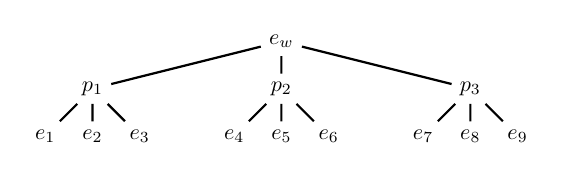
\begin{tikzpicture}   
    [thick,scale=0.4, every node/.style={scale=0.8}]

    \node {$e_w$}
    child {node {$p_1$}
        child {node {$e_1$}}
        child {node {$e_2$}}
        child {node {$e_3$}}
    }    
    child [missing] {}    
    child [missing] {} 
    child [missing] {}        
    child { node {$p_2$}
        child {node {$e_4$}}
        child {node {$e_5$}}
        child {node {$e_6$}}
    }    
    child [missing] {}
    child [missing] {}    
    child [missing] {}    
    child { node {$p_3$}
        child {node {$e_7$}}
        child {node {$e_8$}}
        child {node {$e_9$}}
    };
\end{tikzpicture}

\end{document}